% Number 270
% CVPMA Algebra Units
% Two objects moving, find collision time
% JG

% Watermark
\AddToShipoutPicture*{\BackgroundPic}

\addtocounter {ProbNum} {1}

%\begin{floatingfigure}[r]{.3\textwidth}
%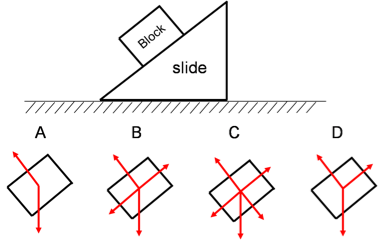
\includegraphics[scale=.4]{/Users/jgates/desktop/latex/pics/incline3.png}
%\end{floatingfigure}
 
{\bf \Large{\arabic{ProbNum}}} Instead of waiting for a soccer pass to come to you, moving towards the ball can greatly increase your chances of not having the ball stolen.  A pass is made to you from 25 meters away, with a speed of ${13~\tfrac{m}{s}}$.  After a .4 second pause (your reaction time), you begin running towards the ball at ${5~\tfrac{m}{s}}$.

\bigskip
What issues might make a CVPM model of this situation less than faithful to the real situation?

\vspace{30mm}
Where (at what position) will you receive the pass?

%\begin{center}
%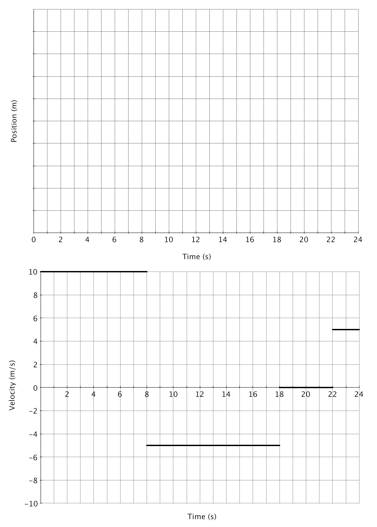
\includegraphics[scale=.77]{/Users/jgates/desktop/latex/pics/vtoxgraph1.png}
%\end{center}
 
\vfill

\newpage